\section{Methodology}

\subsection{Profiling}
When making an effort to accelerate a model like DALES, one should first figure out which parts of the code contribute the most to the wall clock time. This act is called profiling, and there are numerous tools available that serve this purpose. One tool in particular that is very well suited for GPU applications, is NVIDIA's Nsight Systems (NSys) \citep{nvidiaNVIDIANsightSystems}. NSys automatically tracks CPU-GPU interactions, such as data transfer, and GPU utilization, but does not track CPU utilization. To track CPU activity, a custom timer module based on the NVIDIA Tools Extension (NVTX) library is used, allowing the programmer to annotate sections of their code to measure their wall-clock time. 

\begin{figure}[H]
    \centering
    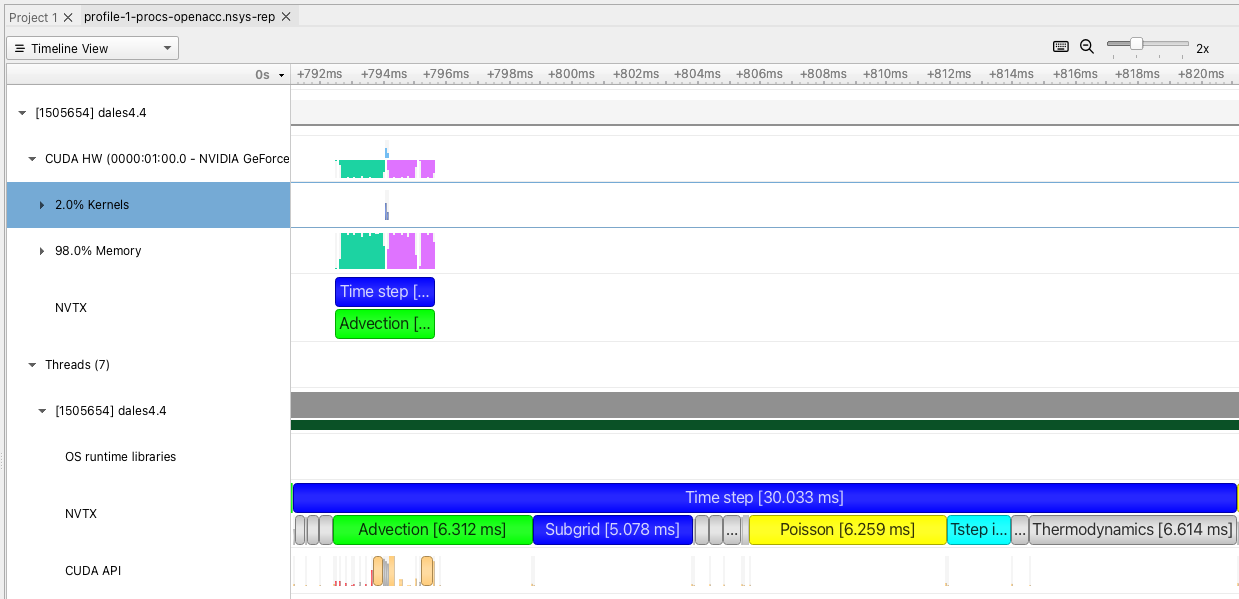
\includegraphics[width=0.9\textwidth]{doc/images/profiles/nsys.png}
    \caption{}
    \label{fig:my_label}
\end{figure}

\subsection{OpenACC}
Computationally expensive parts of DALES will be offloaded to the GPU using OpenACC. OpenACC provides a range of \emph{compiler directives}, which can be used to offload loops to the GPU. An example of such a loop, decorated with an OpenACC directive, can be found in \autoref{listing:accloop}. This directive-based approach offers multiple benefits over the traditional, lower-level programming models such as CUDA and OpenCL \citep{herdmanAcceleratingHydrocodesOpenACC2012}:

\begin{itemize}
    \item Productivity: OpenACC requires minimal addition of lines of code to an existing codebase. This makes it possible for a programmer to accelerate large sections of a program in a relatively short amount of time. 
    \item Single source code: CUDA and OpenCL require the programmer to rewrite existing code into ``\emph{compute kernels}'' that are executed on the GPU. If it is desired that a program is still able to run on CPU's, two versions of the same program have to be maintained: one version for CPU's and one version for GPU's. Needless to say, this is more error-prone than a single source code. As OpenACC directives are essentially just comments in the code, the programmer can add them to the existing CPU code. The same code can then be compiled for execution on both GPU's and CPU's, and the OpenACC directives will simply be ignored for the latter.
\end{itemize}

\begin{listing}[H]
\begin{minted}{fortran}
!$acc parallel loop
do k = 1, kmax
    do j = 1, jmax
        do i = 1, imax
            c(i,j,k) = a(i,j,k) + b(i,j,k)
        end do
    end do
end do
\end{minted}
\caption{Example of a Fortran loop decorated with an OpenACC directive. The directive \texttt{!\$acc parallel loop} tells the compiler that the following loop can be executed in parallel}
\label{listing:accloop}
\end{listing}

\subsection{Solving the Poisson equation}

In DALES, a solution for the pressure $\pi$ is obtained by solving the following Poisson equation:

\begin{equation}
    \frac{\partial^2 \pi}{\partial x_i^2} = \frac{\partial }{\partial x_i} \left( - \frac{\partial \overline{u}_i \overline{u}_j}{\partial x_j} + \frac{g}{\theta_0}\overline{\theta}_v\delta_{i3} + \mathcal{F}_i - \frac{\partial \tau_{ij}}{\partial x_j} \right) \label{eq:pressure}
\end{equation}

 DALES provides two methods to solve this equation: 1) using Fast Fourier Transforms (FFT's), 2) using iterative solvers. Among these, the FFT-based solver is the most efficient. DALES has the ability to use the highly optimized Fastest Fourier Transform in the West (FFTW) library \citep{FFTW97}. FFTW is not capable of running on GPU's, however. NVIDIA provides a FFT library in their HPC SDK, which has a similiar interface as the FFTW library, making the porting straightforward. 

\subsection{Verification}
Modifying source code brings the possibility of introducing bugs in the code. While OpenACC requires minimal rewriting of source code, some rewriting may be inevitable. Hence, the updated source code needs to be validated against the original, unmodified code to check whether the program logic has changed. To this end, one would usually assert whether the end result of the two programs are equal or not. This approach is not feasible for a simulation of a turbulent boundary layer, however, as weather-like simulations are subject to chaos. A small perturbation of some prognostic variable can lead to vastly different results in the end. One source of such a perturbation can be the rounding off done by the computer. Even when using the exact same initial conditions, the point-wise end results of two runs may still differ, while each of the solutions could still be considered correct. A better approach would be to look at averaged statistics of several variables. 

